%%%%%%%%%%%%%%%%%%%%%%%%%%%%%%%%%%%%%%%%%
% NIWeek 2014 Poster by T. Reveyrand
% www.microwave.fr
% http://www.microwave.fr/LaTeX.html
% ---------------------------------------
% 
% Original template created by:
% Brian Amberg (baposter@brian-amberg.de)
%
% This template has been downloaded from:
% http://www.LaTeXTemplates.com
%
% License:
% CC BY-NC-SA 3.0 (http://creativecommons.org/licenses/by-nc-sa/3.0/)
%
%%%%%%%%%%%%%%%%%%%%%%%%%%%%%%%%%%%%%%%%%

%----------------------------------------------------------------------------------------
%	PACKAGES AND OTHER DOCUMENT CONFIGURATIONS
%----------------------------------------------------------------------------------------

\documentclass[a0paper,portrait]{baposter}

\usepackage[font=small,labelfont=bf]{caption} % Required for specifying captions to tables and figures
\usepackage{booktabs} % Horizontal rules in tables
\usepackage{relsize} % Used for making text smaller in some places

\usepackage{amsmath,amsfonts,amssymb,amsthm} % Math packages
\usepackage{eqparbox}

\usepackage{textcomp}
\usepackage{multicol}
\usepackage{wrapfig} % Allows wrapping text around tables and figures

\graphicspath{{figures/}} % Directory in which figures are stored

 %\definecolor{bordercol}{RGB}{40,40,40} % Border color of content boxes
 \definecolor{bordercol}{RGB}{186,215,230} % Border color of content boxes

 \definecolor{headercol1}{RGB}{0,102,51} % Background color for the header in the content boxes (left side)
\definecolor{headercol2}{RGB}{0,102,51} 
% \definecolor{headercol2}{RGB}{120,120,120} % Background color for the header in the content boxes (right side)
 \definecolor{headerfontcol}{RGB}{256,256,256} % Text color for the header text in the content boxes
 %\definecolor{boxcolor}{RGB}{210,235,250} % Background color for the content in the content boxes
\definecolor{boxcolor}{RGB}{250,250,250}

\begin{document}
\background{}
%\background{ % Set the background to an image (background.pdf)
%\begin{tikzpicture}[remember picture,overlay]
%\draw (current page.north west)+(-2em,2em) node[anchor=north west]
%{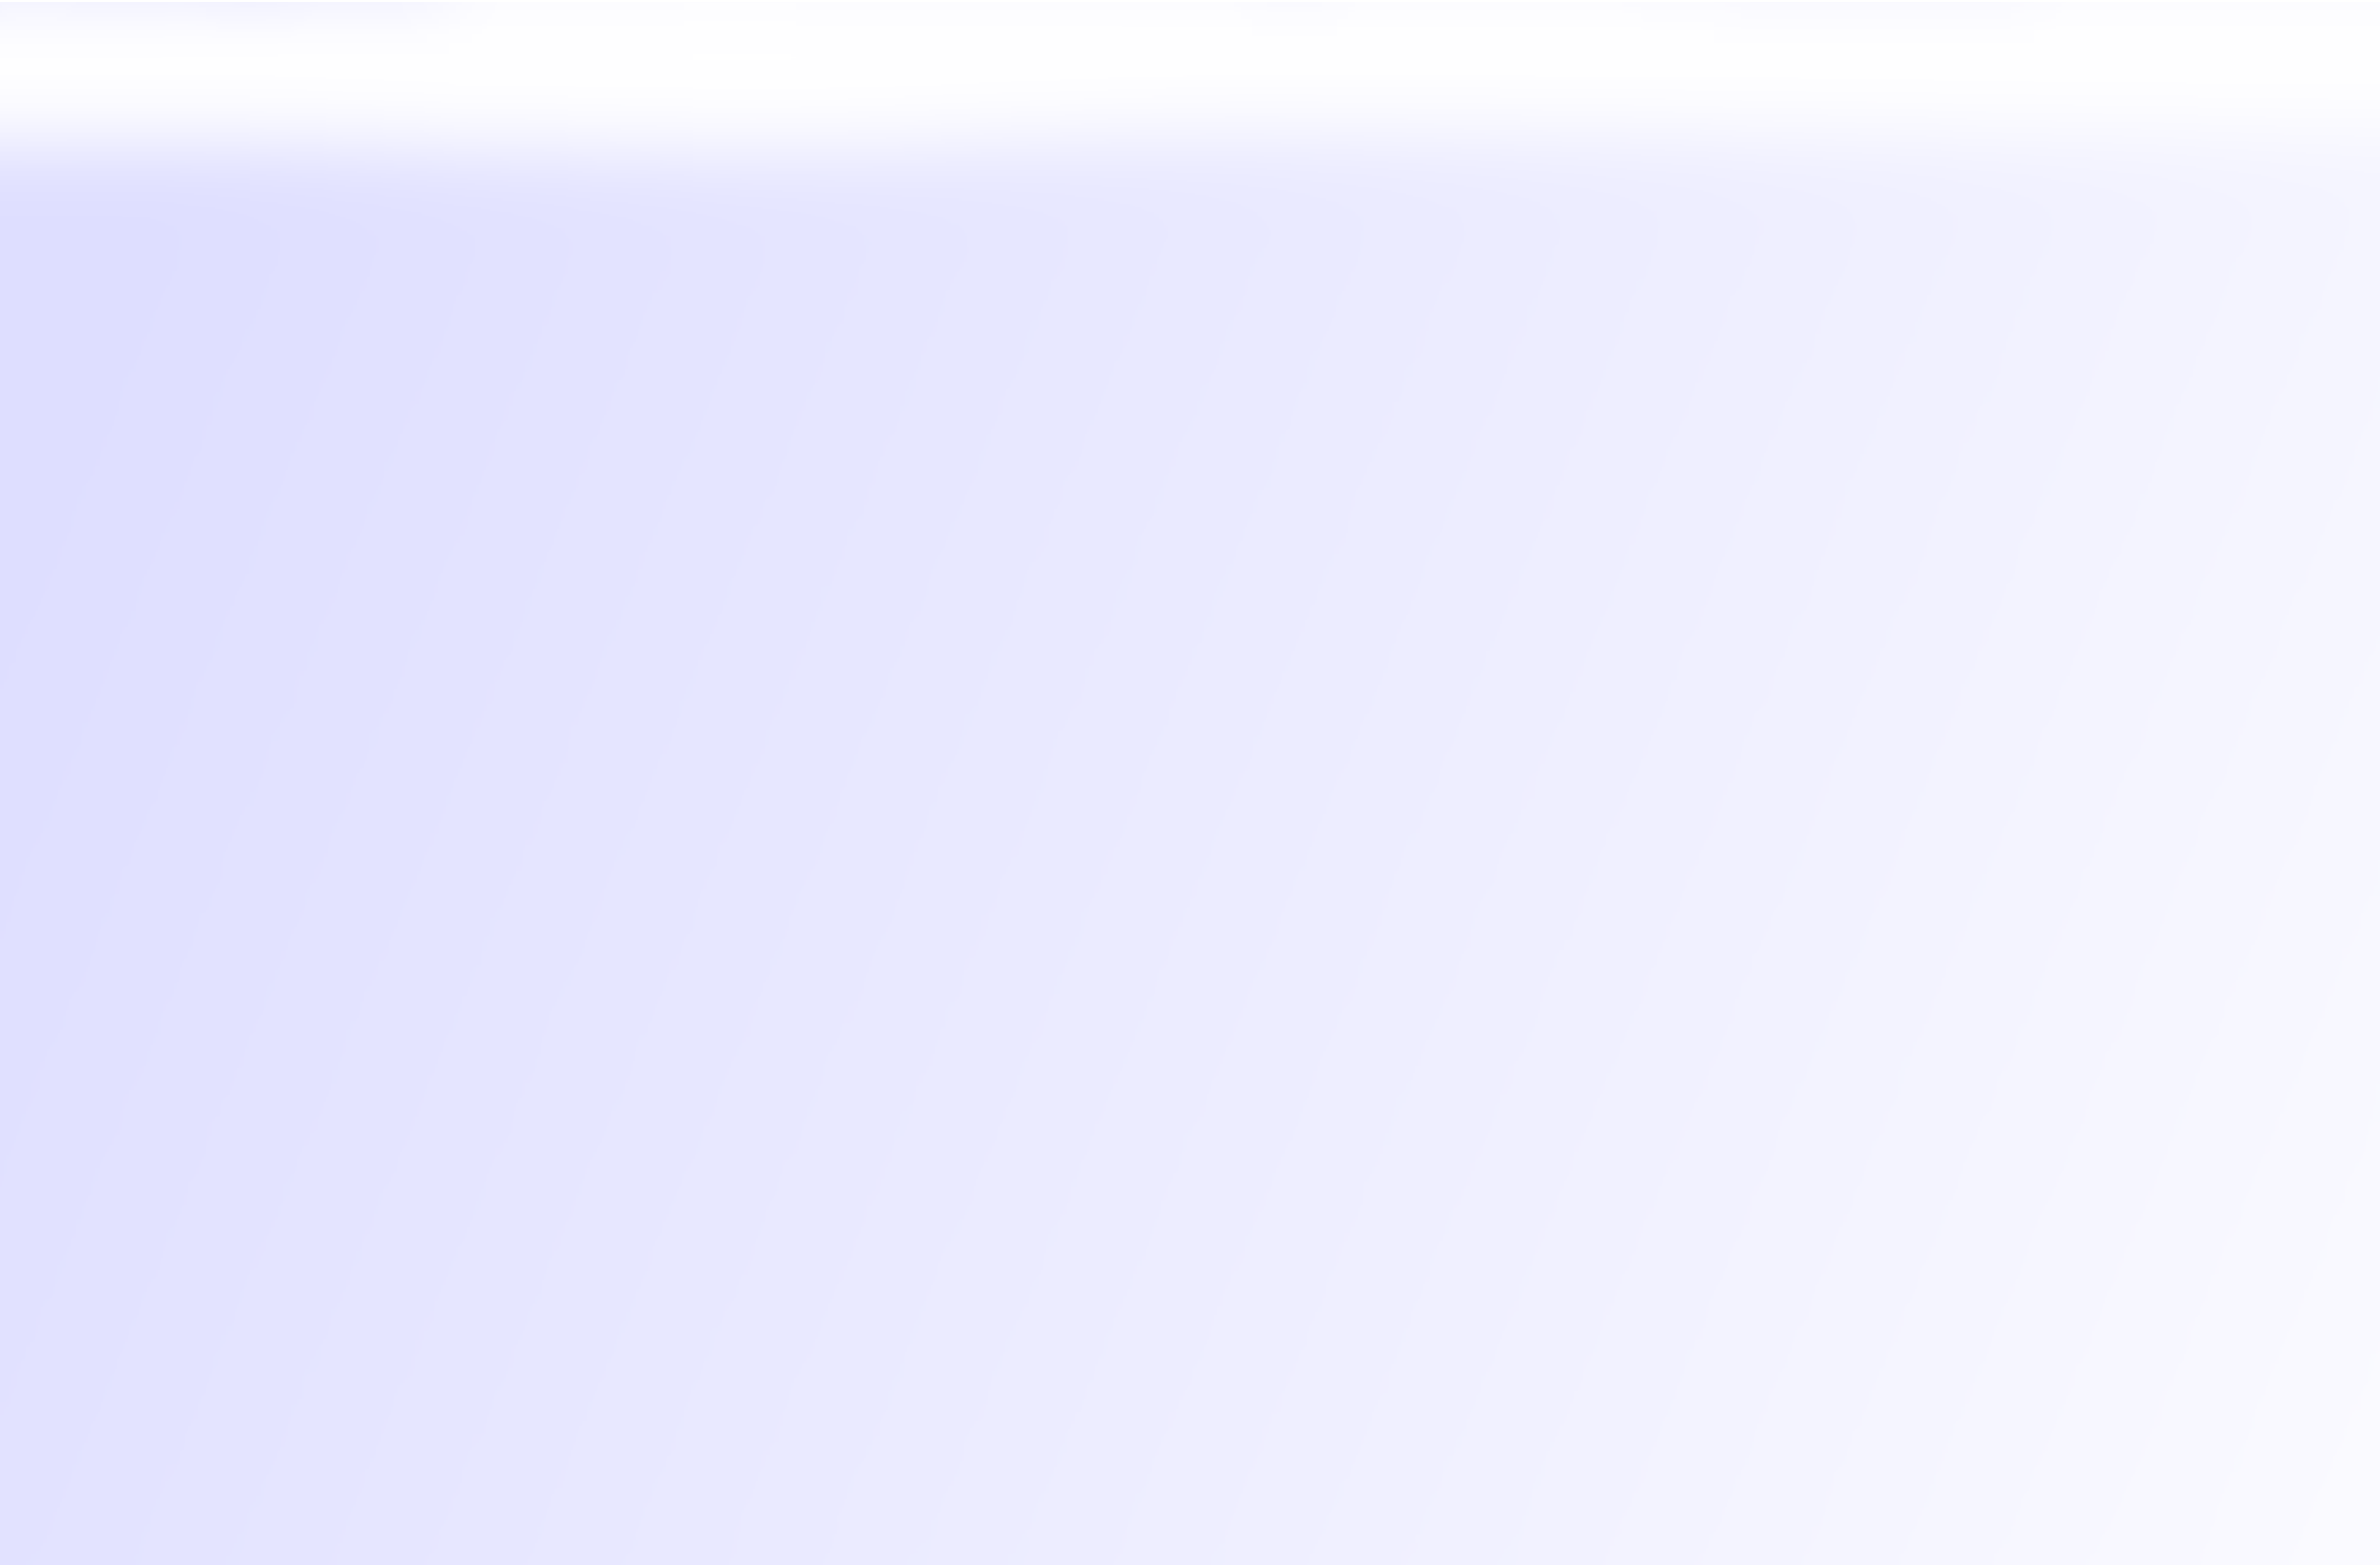
\includegraphics[height=1.1\textheight]{background}};
%\end{tikzpicture}
%}

\begin{poster}{
grid=false,
borderColor=bordercol, % Border color of content boxes
headerColorOne=headercol1, % Background color for the header in the content boxes (left side)
headerColorTwo=headercol2, % Background color for the header in the content boxes (right side)
headerFontColor=headerfontcol, % Text color for the header text in the content boxes
boxColorOne=boxcolor, % Background color for the content in the content boxes
headershape=roundedright, % Specify the rounded corner in the content box headers
headerfont=\Large\sf\bf, % Font modifiers for the text in the content box headers
textborder=rectangle,
background=user,
headerborder=open, % Change to closed for a line under the content box headers
boxshade=plain
}
{
\includegraphics[scale=0.10]{logo_davidson.png}}
%
%----------------------------------------------------------------------------------------
%	TITLE AND AUTHOR NAME
%----------------------------------------------------------------------------------------
%
{ \bf  \huge {A Streamlined Python Framework for AT-TPC Data Analysis} }
%\Large \it A} % Poster title
{\vspace{0.3em} \smaller Jack Taylor and Dr. Michelle Kuchera \\  % Authors
  
\smaller \it {Department of Physics, Davidson College, Davidson, NC 28035}} % Author email addresses
{
\includegraphics[scale=0.3]{nscl_logo.png}} % University/lab logo

%----------------------------------------------------------------------------------------
%	ABSTRACT
%----------------------------------------------------------------------------------------
\headerbox{Abstract}{name=abstract,column=0,row=0, span=3}{
\small{Data-analysis software for the Active-Target Time Projection Chamber (AT-TPC) at the National Superconducting Cyclotron Laboratory (NSCL) was documented and used to analyze unbound states in Argon-40 ($^{40}$Ar). NSCL is a national user facility funded by the National Science Foundation that provides rare isotope beams to researchers around the world to study cutting-edge nuclear physics phenomena. Rare isotope beams are produced, accelerated, and delivered to various experimental setups, each with their own physics motivations. One such setup is the AT-TPC, a gas-filled detector that acts as both the detector and target for high-efficiency detection of low-intensity, exotic nuclear reactions. The pytpc framework is a Python package for analyzing AT-TPC data and was developed for the analysis of $^{46}$Ar(p, p) data. The existing software was used to analyze data produced by the $^{40}$Ar(p, p) experiment that ran in August, 2015. Usage of the package was documented in an analysis manual both to improve analysis steps and aid in the work of future AT-TPC users. Software features and analysis methods in the pytpc framework will be presented along with the $^{40}$Ar results.
}
}
%----------------------------------------------------------------------------------------
%	THE AT-TPC
%----------------------------------------------------------------------------------------
\headerbox{The Active-Target Time Projection Chamber}{name=attpc,column=1,row=1,span=2,below=abstract}
{\small{KuPol is contributing to estimate the location for the high energy emission on these AGNs and to study potential spectral fluctuations that may arise during the flaring events. The uncertainty on the degree of correlation between different energies reduces when the data span for long periods and is rich in sampling, hence the rationale for this program and we therefore advocate for similar observing modes at other frequencies.}
%\begin{wrapfigure}{l}{60mm}
\begin{center}
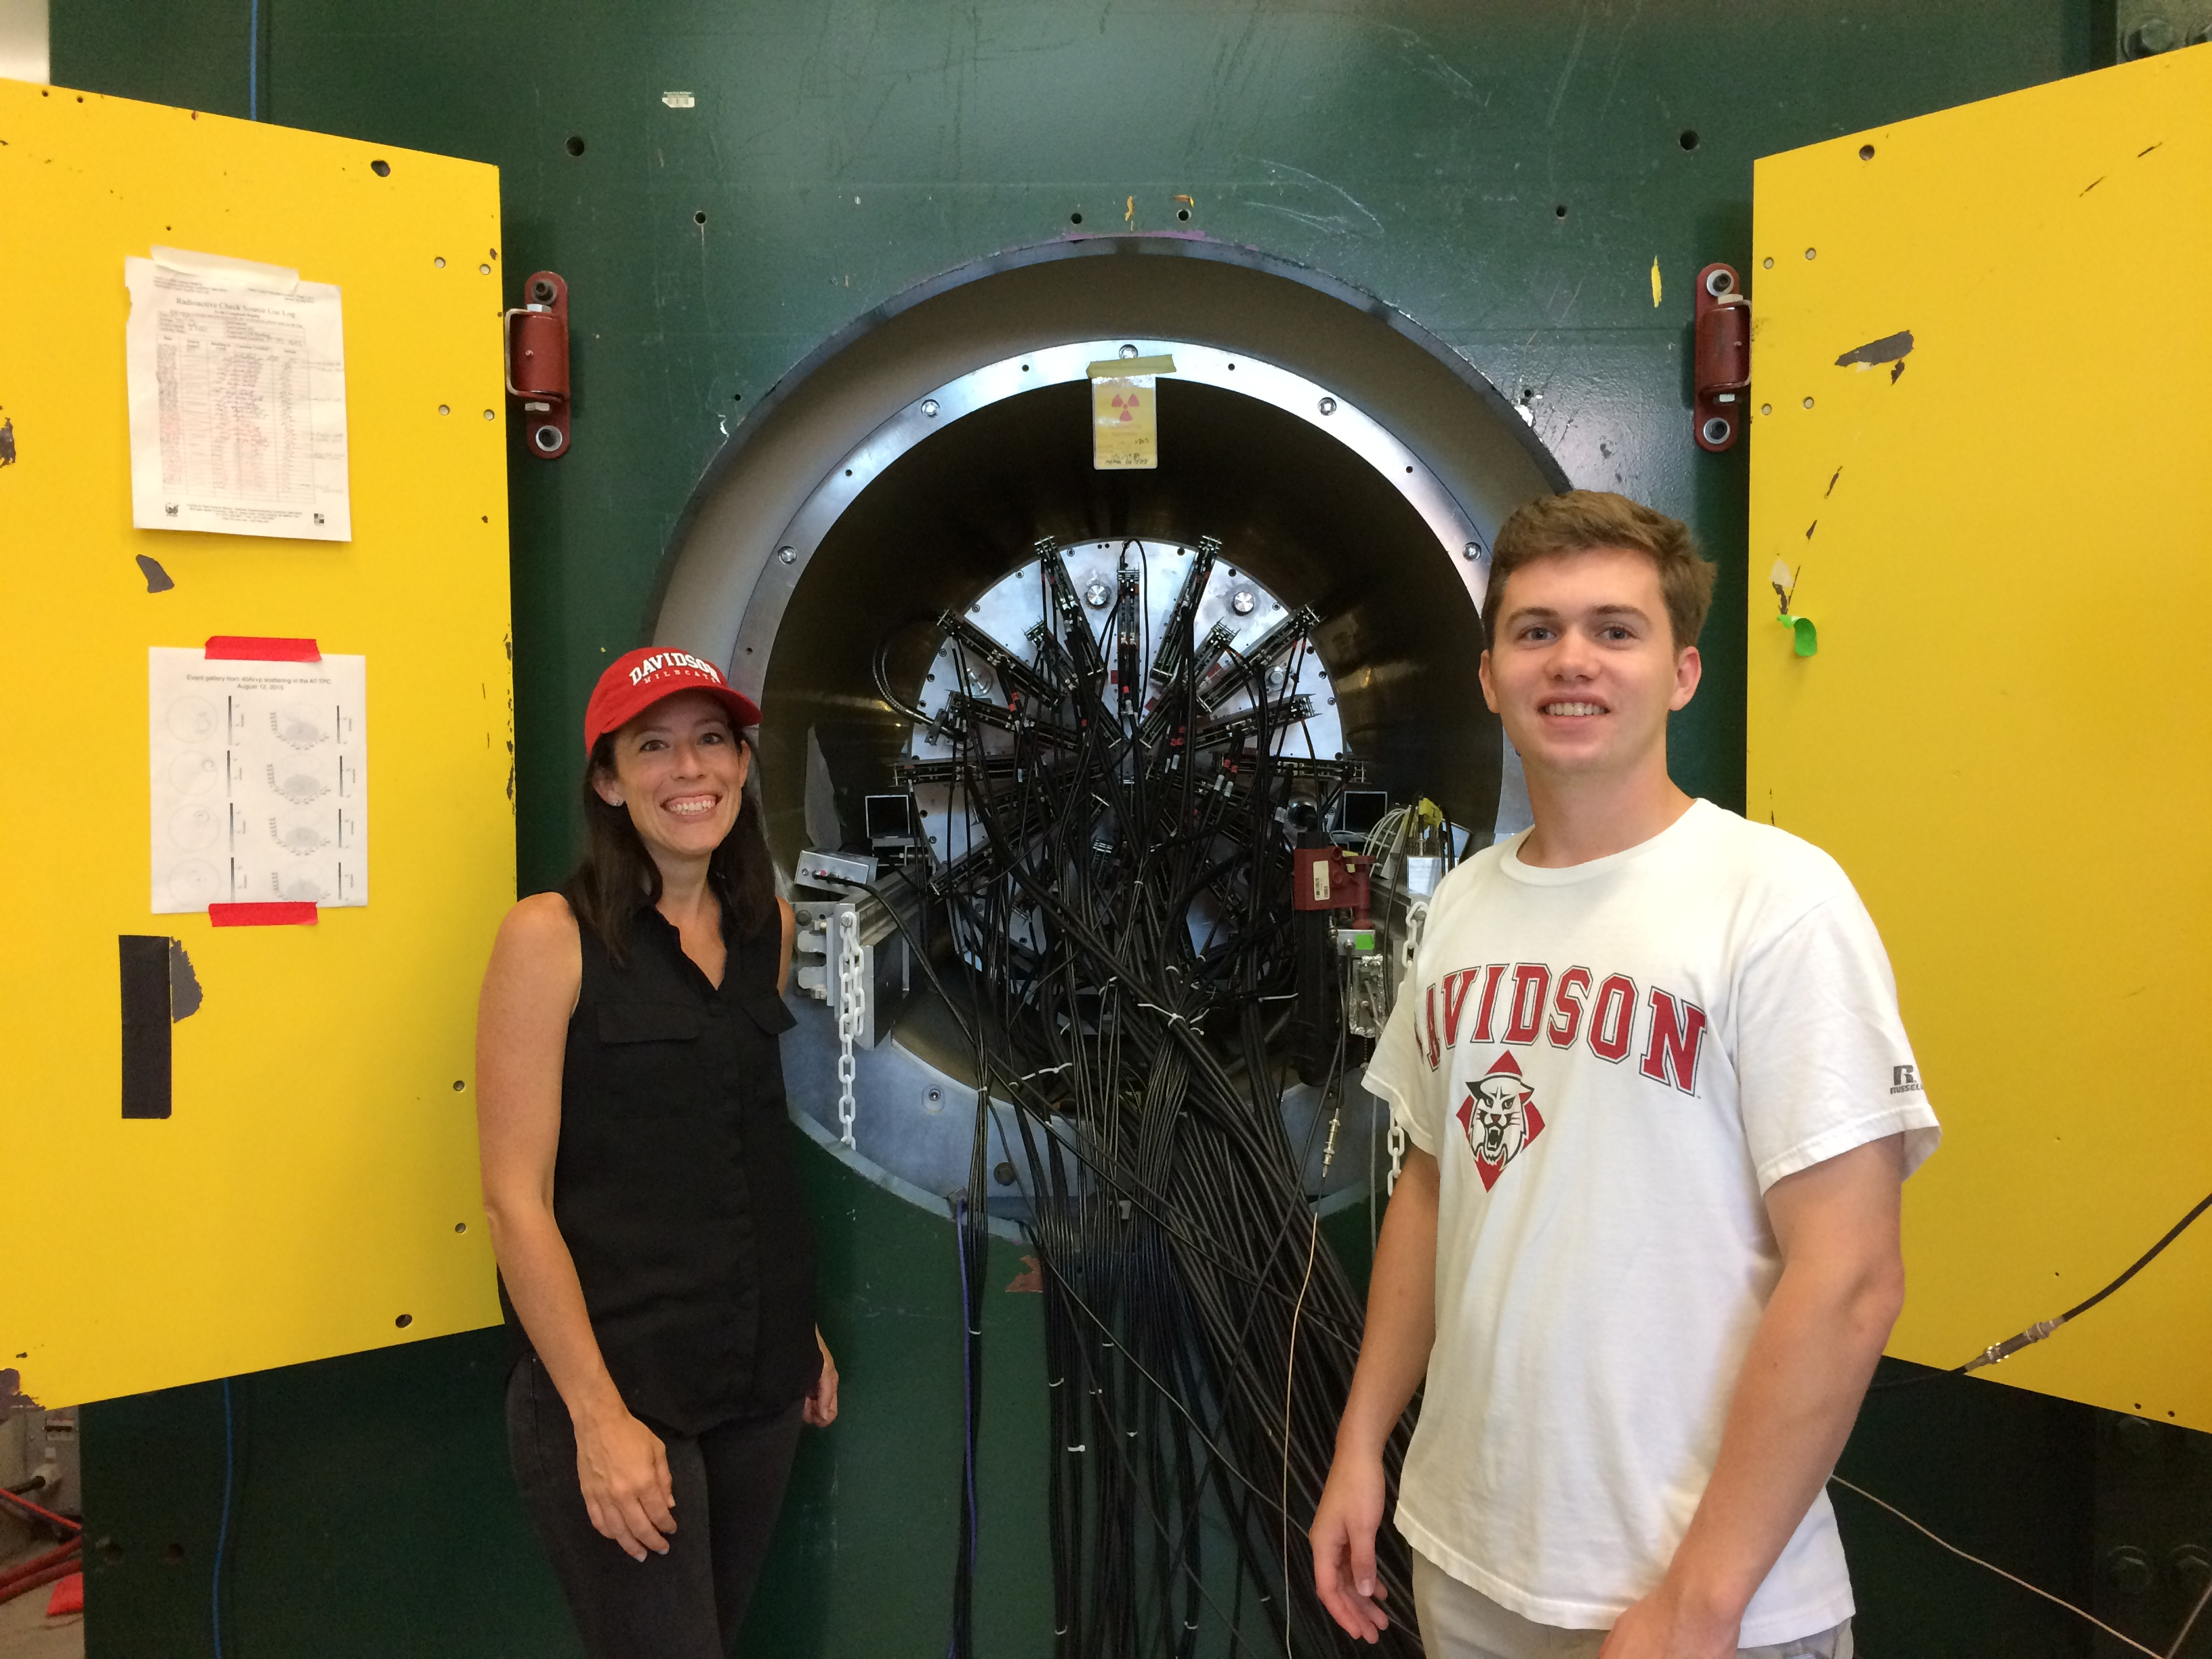
\includegraphics [height=30mm]{michigan_trip.jpg} %[height=36mm, width=60mm] {michigan_trip.jpg}
\hspace{0.2cm}
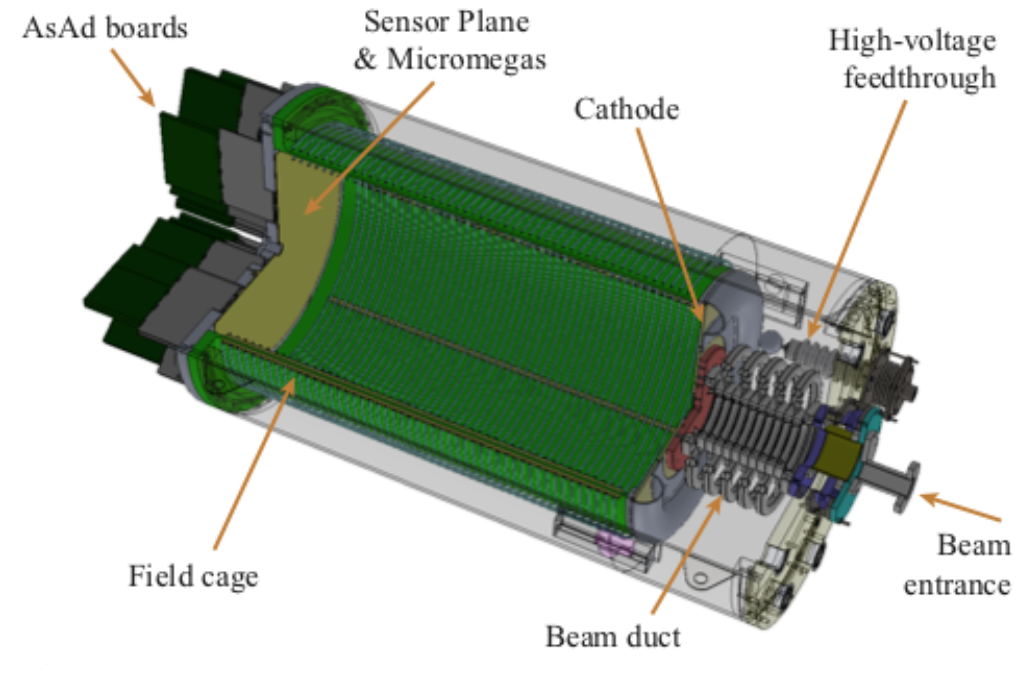
\includegraphics [height=30mm] {attpc.png}
\end{center}
\textbf{Figure 1.} Left side, diagram analog instrument. Right side, diagram digital instrument.\\
%\end{wrapfigure}
\small{The KuPol instrument is a dual-beam receiver for the 40m telescope at OVRO. It is, in fact, a hybrid of two separate instruments called the analog and the digital instrument. The \textbf{Analog Instrument} is a dual-polarization, beam-differencing radiometer that is designed to produce identical data to the previous Ku-band, instrument that KuPol replaces. It is composed by the Cryostat, the Cold Plate, and UBE. The \textbf{Digital Instrument} is a digital spectropolarimeter that processes the band between 13 to 18 GHz in 500 MHz wide chunks with ∼8 MHz resolution. In this instrument is performed the signal distribution, downconversion, digitization and processing, and data readout and archiving.}

}
%----------------------------------------------------------------------------------------
%	Motivation
%----------------------------------------------------------------------------------------
\headerbox{Motivation}
{name=motivation,column=0,row=1,below=abstract}
{\small{The calibration is achieved by measuring the isolation parameter, $\alpha$, at different angles.}
\small{\textbf{Figure 2.} Plot comparing before/after $\alpha$ for 2016-01-18 Digital Model Calibration.\\
For the calibration procedure, we take spectra of quantities derived from voltages in each bin after the FFT with the noise diode on, and then with the noise diode off. We use this data to adjust for the varying gain and phase of the four RF chains, and hence calibrate the receiver output. The calibration procedure instrument is a three-step process, requiring three different firing of the noise diode, each with their own set of calculations.\\
\textbf{1. Gain Correction.} We calculate the gain correction for each RF channel. We assume that the noise diode injects a flat spectrum, and calculate the gain correction coefficients $B_{j}$ for $j=1...4$.}
}
%----------------------------------------------------------------------------------------
%	40AR ANALYSIS
%----------------------------------------------------------------------------------------
\headerbox{Analysis of the $^{40}$Ar Beam Experiment Data}{name=analysis,span=2,column=1,row=1, below=attpc}{
\small{The Power Spectral Density (PSD) of a signal is the spectral decomposition of a signal into different frequency components, as a function of power at each frequency bin.\\
The PSD is usually estimated by means of an FFT, and it can be used to characterize the time variability of the blazar flux. The analysis requires regularity in the signal sampling, which is seldom the case. The PSD can also be estimated by a periodogram, which is the convolution between a window function and the signal. We are trying Blackman-Harris window function in order to minimize the spectral sidelobes introduced in the analysis.}
\begin{center}
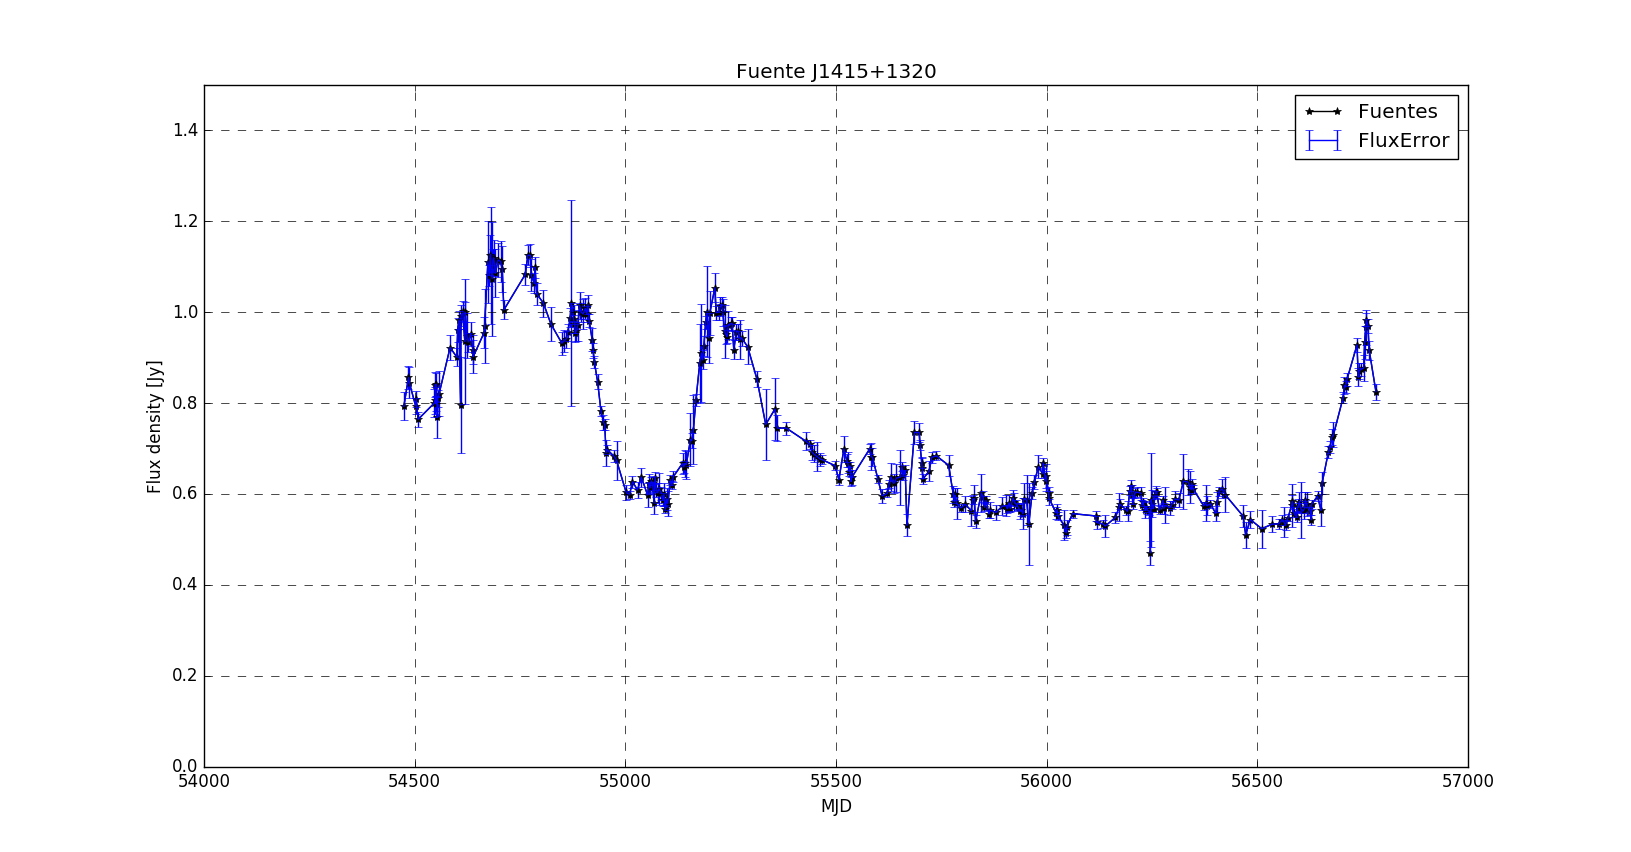
\includegraphics [height=20mm, width=50mm] {curvaJ1415.jpg}
\hspace{.5cm}
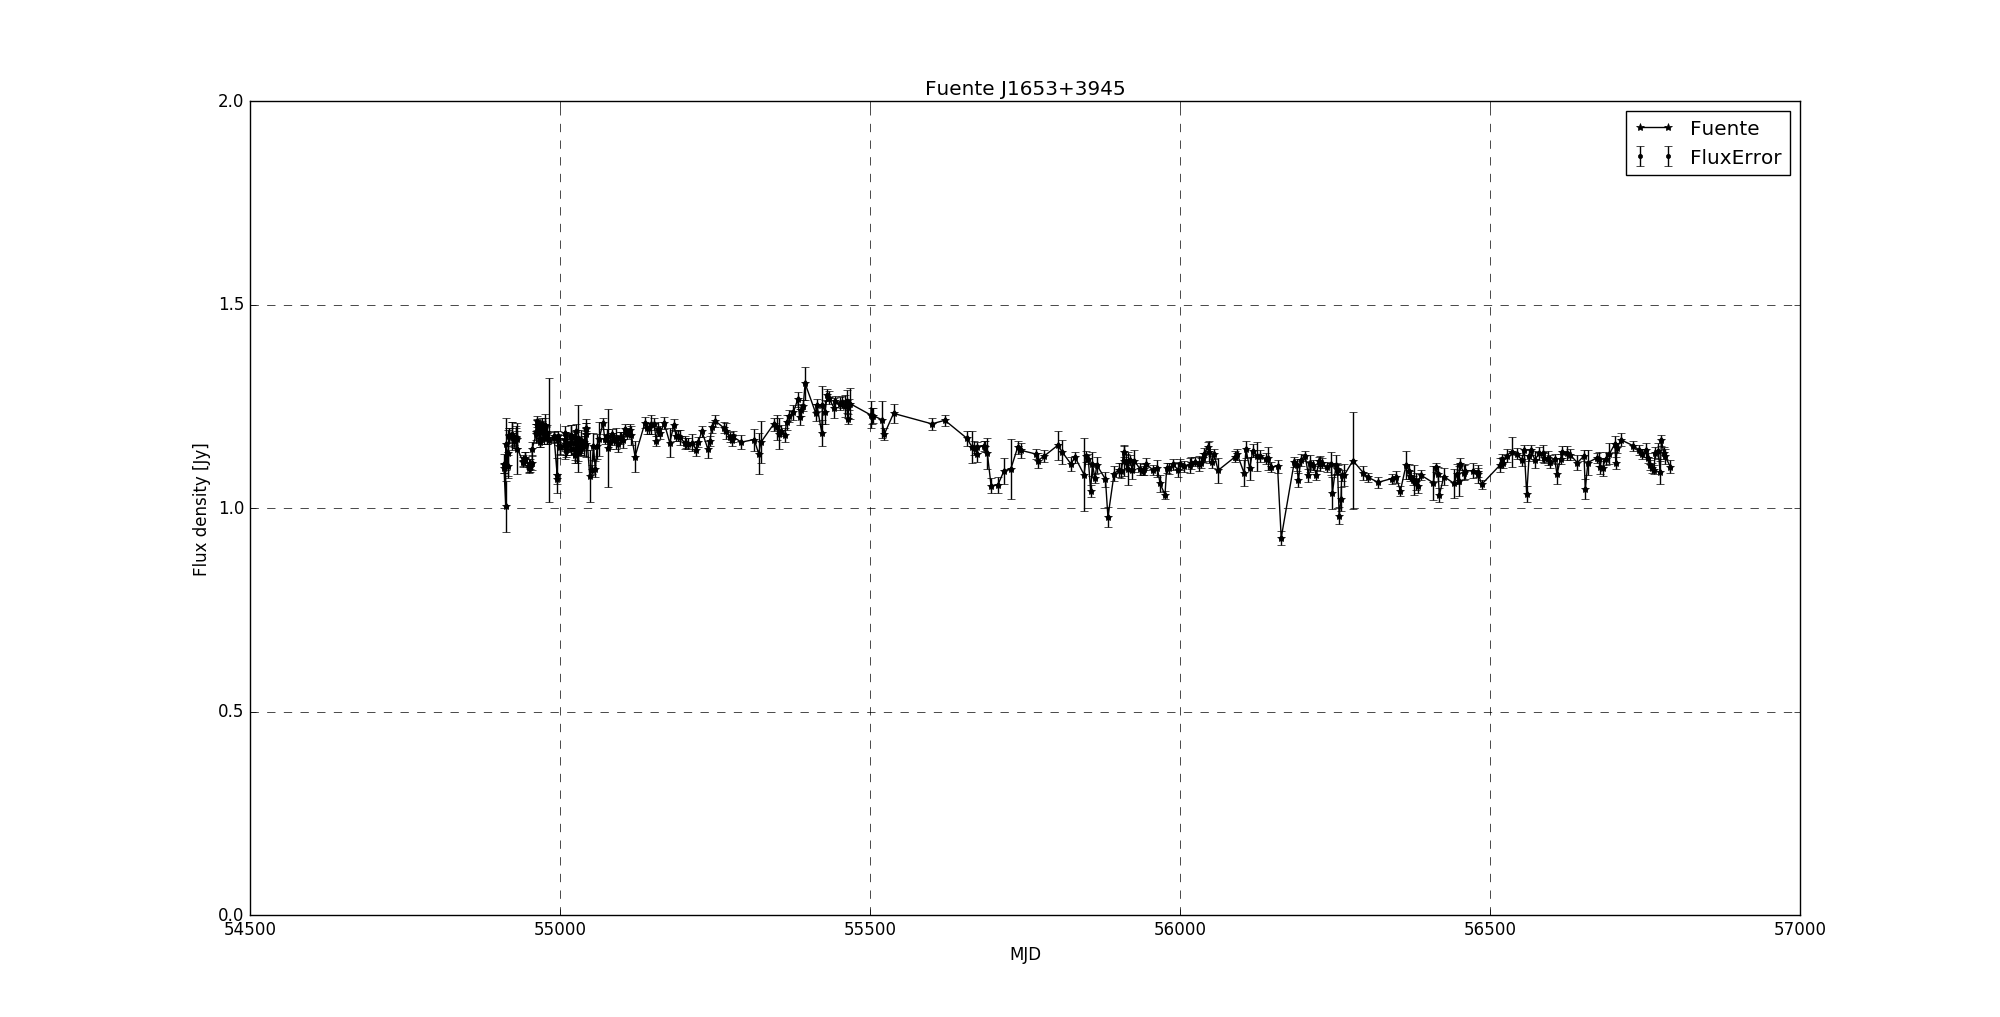
\includegraphics [height=20mm, width=50mm] {curvaJ1653.jpg}
\end{center}
\small{\textbf{Figure 3.} The first and second plot correspond the sources of J1415+1320 and J1653+3945, respectively, observed by the OVRO program.}\\
The next step to determine the PSD, is to calculate the Fourier Transform of the window function and the curve separately and convolve, which is analogous to convolve the signal with the window function and apply Transform.
\begin{center}
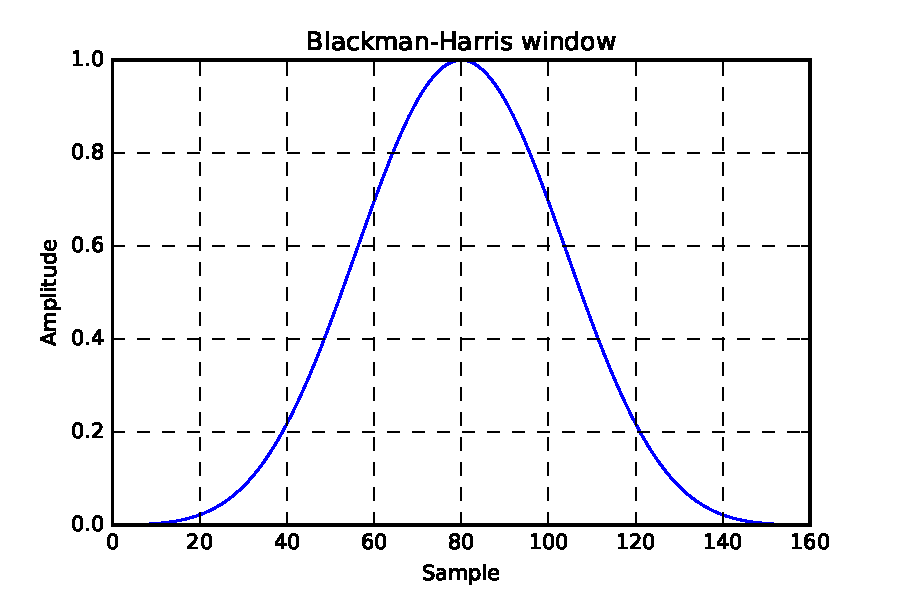
\includegraphics [height=30mm, width=43mm] {BH.pdf}
\hspace{.3cm}
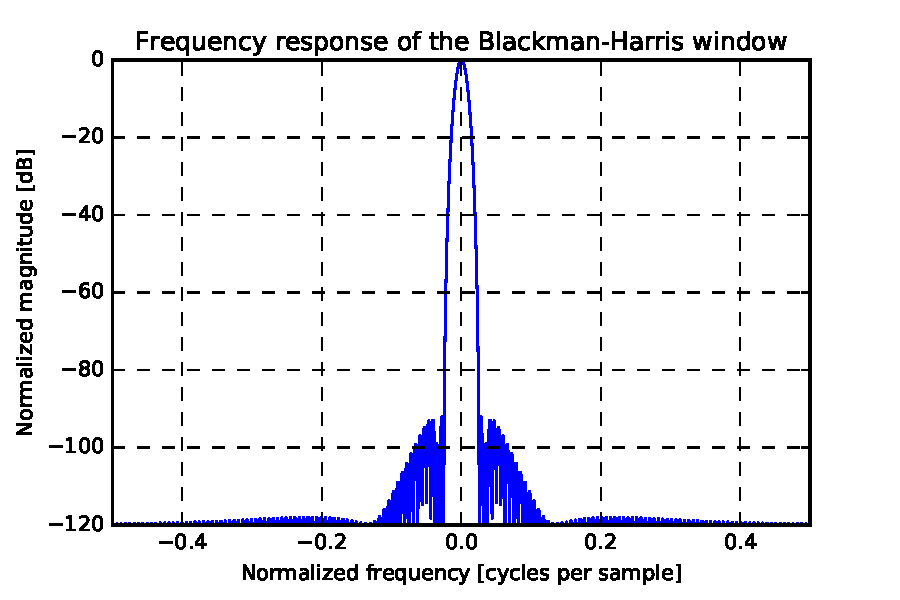
\includegraphics [height=30mm, width=48mm] {FFTBH.pdf}
\hspace{.3cm}
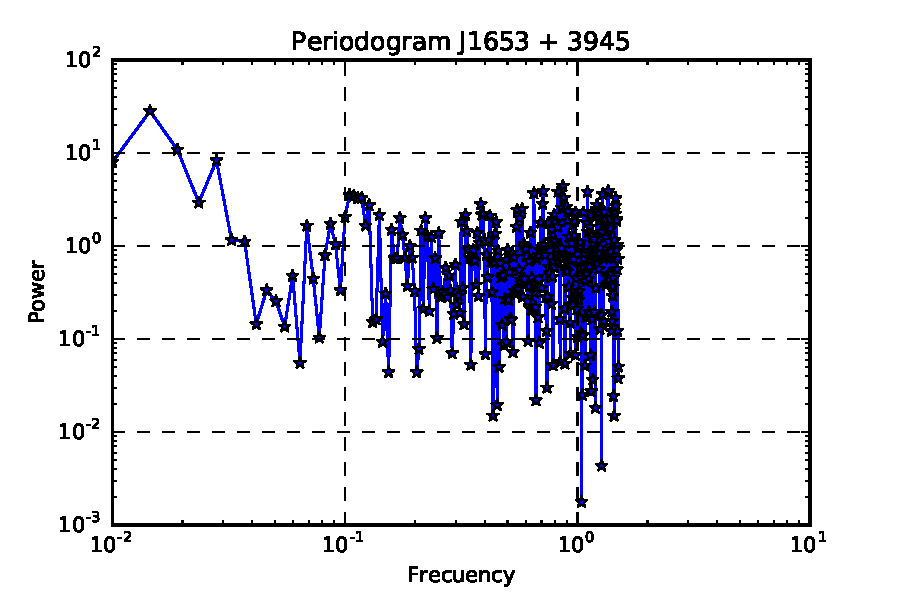
\includegraphics [height=30mm, width=43mm] {FFTcurva_2.pdf}
\end{center}
\small{\textbf{Figure 4.} The first and second plot correspond the  Blackman-Harris window function, without FFT and with FFT, respectively. The third plot is FFT of light curve J1653+3945, calculated exclusively by Lomb-Scargle periodogram.}
}

%----------------------------------------------------------------------------------------
%	CONCLUSION - FUTURE
%----------------------------------------------------------------------------------------
\headerbox{Conclusion and Future Work}{name=conclusion,column=1,below=analysis,span=2}
{\small{ With the PSD analysis and by looking for correlations in the variability, we hope to better understand the emission mechanisms at the hearts of Active Galactic Nuclei. The work is under development and we are in search of the best method to estimate the PSD. On the other hand we have presented and defined the KuPol calibration method. From this in the coming weeks we will obtain calibration results of the 40m receiver. }
}
%----------------------------------------------------------------------------------------
%	REFERENCES
%----------------------------------------------------------------------------------------
\headerbox{References}{name=references,column=0,above=bottom,span=1}{

}
%----------------------------------------------------------------------------------------
%	PYTPC
%----------------------------------------------------------------------------------------
\headerbox{The pytpc Framework}{name=pytpc,column=0,row=2,below=motivation, above=references}{\small{The OVRO 40m Telescope Fermi Blazar Monitoring Program is supported by NASA under awards NNX08AW31G and NNX11A043G, and by the NSF under awards AST-0808050 and AST-1109911.
\begin{center}
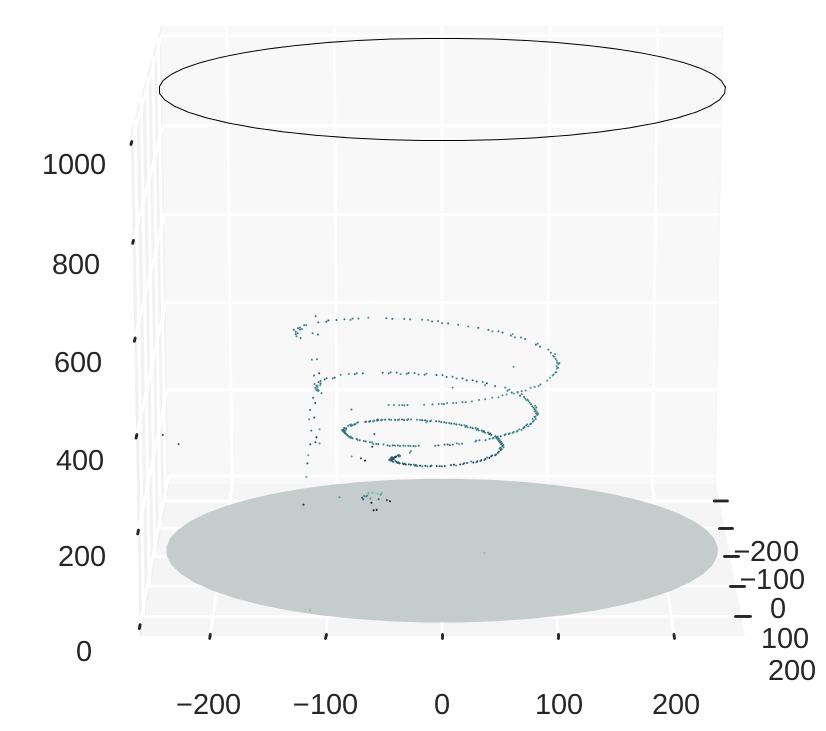
\includegraphics[scale=0.15]{chamber_plot.png}
\end{center}
\small{\textbf{Figure 100.} An example of a proton track event in the AT-TPC chamber from the $^{40}$Ar experiment.}\\
}
} 

\end{poster}
\end{document}
